\documentclass[border=10pt]{standalone}
\usepackage{tikz}
\usetikzlibrary{shapes.geometric, arrows.meta, positioning, fit, backgrounds, calc}

\tikzset{
    block/.style={rectangle, draw, fill=blue!20, text width=6em, text centered, rounded corners, minimum height=3em},
    smallblock/.style={rectangle, draw, fill=blue!15, text width=4em, text centered, rounded corners, minimum height=2em, font=\small},
    wideblock/.style={rectangle, draw, fill=green!20, text width=10em, text centered, rounded corners, minimum height=3em},
    storage/.style={rectangle, draw, fill=yellow!20, text width=5em, text centered, minimum height=2.5em},
    process/.style={rectangle, draw, fill=orange!20, text width=7em, text centered, rounded corners, minimum height=3em},
    sbox/.style={rectangle, draw, fill=red!20, text width=3em, text centered, minimum height=2em, font=\small},
    decision/.style={diamond, draw, fill=green!20, text width=4em, text badly centered, inner sep=0pt},
    line/.style={draw, -Latex, thick},
    dashedline/.style={draw, -Latex, thick, dashed},
    bigbox/.style={rectangle, draw, thick, fill=gray!10, rounded corners, inner sep=10pt},
}

\begin{document}

% ============================================================================
% Figure 1: On-the-Fly Key Expansion Module
% ============================================================================
\begin{tikzpicture}[node distance=1.5cm, auto]

    % Title
    \node[font=\Large\bfseries] (title) at (0, 8) {AES-128 On-the-Fly Key Expansion Module};

    % Input
    \node[storage] (masterkey) at (0, 6) {Master Key\\[127:0]};

    % Current window
    \node[storage] (w0) at (-4, 4) {w0\\[31:0]};
    \node[storage] (w1) at (-1.5, 4) {w1\\[31:0]};
    \node[storage] (w2) at (1.5, 4) {w2\\[31:0]};
    \node[storage] (w3) at (4, 4) {w3\\[31:0]};

    % Window box
    \node[bigbox, fit=(w0) (w1) (w2) (w3), label=above:Current 4-Word Window (128 bits)] (window) {};

    % RotWord
    \node[process, below=1.5cm of w3] (rotword) {RotWord\\Rotation};

    % SubWord S-boxes
    \node[sbox, below=0.8cm of rotword, xshift=-2cm] (sbox0) {S-box\\0};
    \node[sbox, right=0.3cm of sbox0] (sbox1) {S-box\\1};
    \node[sbox, right=0.3cm of sbox1] (sbox2) {S-box\\2};
    \node[sbox, right=0.3cm of sbox2] (sbox3) {S-box\\3};

    \node[bigbox, fit=(sbox0) (sbox1) (sbox2) (sbox3), label=above:SubWord (4 S-boxes)] (subword) {};

    % Rcon
    \node[storage, below=2.5cm of w0] (rcon) {Rcon\\(round)};

    % XOR operations for next round
    \node[process, below=4cm of w0] (tempw0) {temp\_w0\\= w0 $\oplus$ result\\$\oplus$ Rcon};
    \node[process, below=4cm of w1] (tempw1) {temp\_w1\\= w1 $\oplus$ temp\_w0};
    \node[process, below=4cm of w2] (tempw2) {temp\_w2\\= w2 $\oplus$ temp\_w1};
    \node[process, below=4cm of w3] (tempw3) {temp\_w3\\= w3 $\oplus$ temp\_w2};

    % Output MUX
    \node[process, left=2cm of w0] (outmux) {Output\\MUX};
    \node[wideblock, left=1cm of outmux] (roundkey) {round\_key\\[31:0]};

    % Word address
    \node[storage, below=0.5cm of roundkey] (wordaddr) {word\_addr\\[5:0]\\(0-43)};

    % Control signals
    \node[storage, below=0.5cm of wordaddr] (ready) {ready};
    \node[storage, below=0.5cm of ready] (next) {next};
    \node[storage, below=0.5cm of next] (start) {start};

    % Connections
    \draw[line] (masterkey) -- (window);
    \draw[line] (w3) -- (rotword);
    \draw[line] (rotword) -- (subword);
    \draw[line] (subword) -- (tempw0);
    \draw[line] (rcon) -- (tempw0);
    \draw[line] (tempw0) -- (tempw1);
    \draw[line] (tempw1) -- (tempw2);
    \draw[line] (tempw2) -- (tempw3);

    % Feedback loop
    \draw[line] (tempw0) -- ++(0,-0.8) -| ($(w0.south) + (0,-0.3)$) -- (w0.south);
    \draw[line] (tempw1) -- ++(0,-0.8) -| ($(w1.south) + (0,-0.3)$) -- (w1.south);
    \draw[line] (tempw2) -- ++(0,-0.8) -| ($(w2.south) + (0,-0.3)$) -- (w2.south);
    \draw[line] (tempw3) -- ++(0,-0.8) -| ($(w3.south) + (0,-0.3)$) -- (w3.south);

    % Output path
    \draw[line] (w0) -- (outmux);
    \draw[line] (w1) |- (outmux);
    \draw[line] (w2) |- (outmux);
    \draw[line] (w3) |- (outmux);
    \draw[line] (outmux) -- (roundkey);

    % Annotations
    \node[font=\small, text width=8em] at (-6, -1) {Only 128 bits stored\\vs 1408 bits\\(91\% savings)};
    \node[font=\small, text width=8em] at (6.5, 0) {Next round\\keys generated\\combinationally};

\end{tikzpicture}

\newpage

% ============================================================================
% Figure 2: 32-bit AES Datapath Overview
% ============================================================================
\begin{tikzpicture}[node distance=1.2cm, auto]

    % Title
    \node[font=\Large\bfseries] (title) at (0, 10) {AES-128 Core: 32-bit Datapath};

    % Input
    \node[wideblock] (datain) at (0, 8.5) {data\_in [127:0]};

    % State register
    \node[storage] (col0) at (-4, 7) {Col 0\\[127:96]};
    \node[storage] (col1) at (-1.5, 7) {Col 1\\[95:64]};
    \node[storage] (col2) at (1.5, 7) {Col 2\\[63:32]};
    \node[storage] (col3) at (4, 7) {Col 3\\[31:0]};

    \node[bigbox, fit=(col0) (col1) (col2) (col3), label=above:AES State Register [127:0]] (state) {};

    % Column selector
    \node[process, below=1cm of state] (colsel) {Column Selector\\col\_cnt [1:0]};
    \node[storage, below=0.8cm of colsel] (curcol) {Current Column\\[31:0]};

    % SubBytes
    \node[sbox, below=1cm of curcol, xshift=-2.5cm] (sb0) {S-box\\[0]};
    \node[sbox, right=0.3cm of sb0] (sb1) {S-box\\[1]};
    \node[sbox, right=0.3cm of sb1] (sb2) {S-box\\[2]};
    \node[sbox, right=0.3cm of sb2] (sb3) {S-box\\[3]};

    \node[bigbox, fit=(sb0) (sb1) (sb2) (sb3), label={[font=\small]above:SubBytes (4 Shared S-boxes)}] (subbytes) {};

    % Temp state
    \node[wideblock, below=1.5cm of subbytes] (tempstate) {Temp State [127:0]};

    % ShiftRows
    \node[process, below=0.8cm of tempstate] (shiftrows) {ShiftRows\\(Full 128-bit)};

    % Extract shifted column
    \node[storage, below=0.8cm of shiftrows] (shiftcol) {Shifted Col\\[31:0]};

    % MixColumns
    \node[process, below=0.8cm of shiftcol] (mixcols) {MixColumns\\(32-bit)};

    % AddRoundKey XOR
    \node[process, below=0.8cm of mixcols] (addroundkey) {AddRoundKey\\(XOR)};

    % Round key input
    \node[storage, right=3cm of addroundkey] (rkey) {Round Key\\[31:0]};

    % Key expansion box
    \node[wideblock, above=0.8cm of rkey] (keyexp) {Key Expansion\\OTF};
    \node[wideblock, above=0.8cm of keyexp] (keyreg) {Round Key\\Shift Register\\[0:43]};

    \node[bigbox, fit=(keyreg) (keyexp) (rkey), label=above:Key Management] (keymgmt) {};

    % Output
    \node[wideblock, below=1.5cm of addroundkey] (dataout) {data\_out [127:0]};

    % Control FSM
    \node[bigbox, below right=2cm and 1cm of dataout, text width=12em] (fsm) {
        \textbf{Control FSM}\\[0.2cm]
        \small
        • IDLE\\
        • KEY\_EXPAND\\
        • ROUND0\\
        • ENC\_SUB\\
        • ENC\_SHIFT\_MIX\\
        • DEC\_SHIFT\_SUB\\
        • DEC\_ADD\_MIX\\
        • DONE
    };

    % Connections
    \draw[line] (datain) -- (state);
    \draw[line] (state) -- (colsel);
    \draw[line] (colsel) -- (curcol);
    \draw[line] (curcol) -- (subbytes);
    \draw[line] (subbytes) -- (tempstate);
    \draw[line] (tempstate) -- (shiftrows);
    \draw[line] (shiftrows) -- (shiftcol);
    \draw[line] (shiftcol) -- (mixcols);
    \draw[line] (mixcols) -- (addroundkey);
    \draw[line] (rkey) -- (addroundkey);
    \draw[line] (keyexp) -- (rkey);
    \draw[line] (keyreg) -- (keyexp);
    \draw[line] (addroundkey) -- (dataout);

    % Feedback to state
    \draw[line] (addroundkey) -- ++(-4,0) |- ($(state.south) + (-5,-0.5)$) -- ($(state.south) + (-5,0)$);

    % FSM connections
    \draw[dashedline] (fsm) -- (colsel);
    \draw[dashedline] (fsm) -- (dataout);

    % Annotations
    \node[font=\small, text width=7em, align=center] at (-7, 1) {Processes\\1 column\\per cycle};
    \node[font=\small, text width=7em, align=center] at (8.5, 4) {44 words\\stored\\(176 bytes)};
    \node[font=\small, text width=9em, align=center] at (0, -4) {4 cycles per transformation\\$\sim$440-480 cycles total};

\end{tikzpicture}

\newpage

% ============================================================================
% Figure 3: Detailed Round Processing Timeline
% ============================================================================
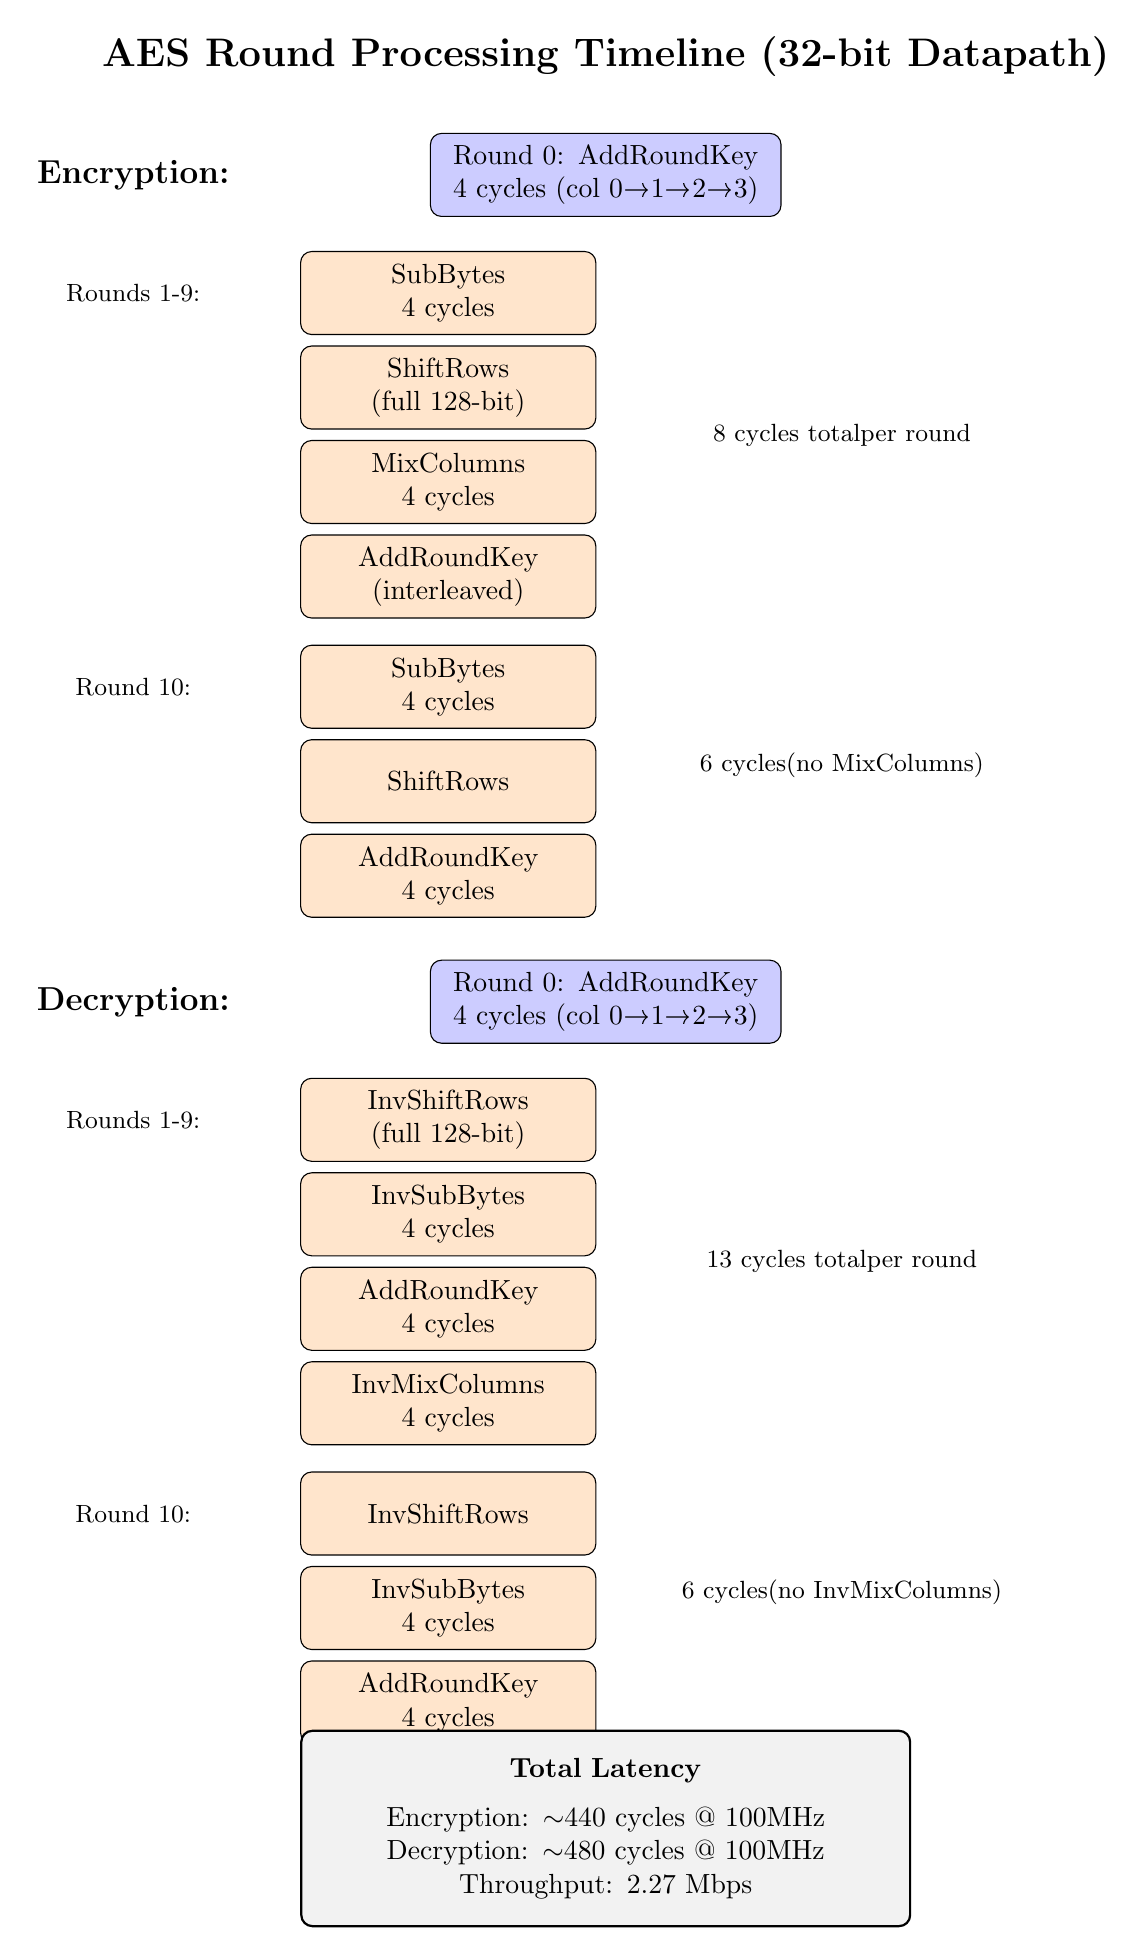
\begin{tikzpicture}[node distance=0.8cm]

    \node[font=\Large\bfseries] (title) at (6, 9) {AES Round Processing Timeline (32-bit Datapath)};

    % Encryption timeline
    \node[font=\large\bfseries] at (0, 7.5) {Encryption:};

    % Round 0
    \node[block, text width=12em] (enc_r0) at (6, 7.5) {Round 0: AddRoundKey\\4 cycles (col 0→1→2→3)};

    % Rounds 1-9
    \node[font=\small] at (0, 6) {Rounds 1-9:};
    \node[process, text width=10em] (enc_sub) at (4, 6) {SubBytes\\4 cycles};
    \node[process, text width=10em] (enc_shift) at (4, 4.8) {ShiftRows\\(full 128-bit)};
    \node[process, text width=10em] (enc_mix) at (4, 3.6) {MixColumns\\4 cycles};
    \node[process, text width=10em] (enc_add) at (4, 2.4) {AddRoundKey\\(interleaved)};

    \node[font=\small] at (9, 4.2) {8 cycles total\\per round};

    % Round 10
    \node[font=\small] at (0, 1) {Round 10:};
    \node[process, text width=10em] (enc_r10_sub) at (4, 1) {SubBytes\\4 cycles};
    \node[process, text width=10em] (enc_r10_shift) at (4, -0.2) {ShiftRows};
    \node[process, text width=10em] (enc_r10_add) at (4, -1.4) {AddRoundKey\\4 cycles};

    \node[font=\small] at (9, 0) {6 cycles\\(no MixColumns)};

    % Decryption timeline
    \node[font=\large\bfseries] at (0, -3) {Decryption:};

    % Round 0
    \node[block, text width=12em] (dec_r0) at (6, -3) {Round 0: AddRoundKey\\4 cycles (col 0→1→2→3)};

    % Rounds 1-9
    \node[font=\small] at (0, -4.5) {Rounds 1-9:};
    \node[process, text width=10em] (dec_shift) at (4, -4.5) {InvShiftRows\\(full 128-bit)};
    \node[process, text width=10em] (dec_sub) at (4, -5.7) {InvSubBytes\\4 cycles};
    \node[process, text width=10em] (dec_add) at (4, -6.9) {AddRoundKey\\4 cycles};
    \node[process, text width=10em] (dec_mix) at (4, -8.1) {InvMixColumns\\4 cycles};

    \node[font=\small] at (9, -6.3) {13 cycles total\\per round};

    % Round 10
    \node[font=\small] at (0, -9.5) {Round 10:};
    \node[process, text width=10em] (dec_r10_shift) at (4, -9.5) {InvShiftRows};
    \node[process, text width=10em] (dec_r10_sub) at (4, -10.7) {InvSubBytes\\4 cycles};
    \node[process, text width=10em] (dec_r10_add) at (4, -11.9) {AddRoundKey\\4 cycles};

    \node[font=\small] at (9, -10.5) {6 cycles\\(no InvMixColumns)};

    % Summary box
    \node[bigbox, text width=20em, align=center] at (6, -13.5) {
        \textbf{Total Latency}\\[0.2cm]
        Encryption: $\sim$440 cycles @ 100MHz\\
        Decryption: $\sim$480 cycles @ 100MHz\\
        Throughput: 2.27 Mbps
    };

\end{tikzpicture}

\end{document}
